\documentclass[mathserif]{beamer}%
%
\xdef\sharedDir{../_shared_}%
\RequirePackage{\sharedDir/styles/slides}%
%
\subtitle{1. Introduction}%
%
\begin{document}%
%
\startPresentation{}%
%
%
\begin{frame}%
\frametitle{What is Optimization?}%
\begin{itemize}%
\item In this unit, we want to get a rough feeling about what \alert{optimization} is.%
\item<2-> So let us start by looking at some examples for optimization problems.%
\end{itemize}%
\end{frame}
%
%
\section{Transportation Planning Example}%
%
%
\begin{frame}[t]\relax\frametitle{Transportation Planning: Task}%
\begin{itemize}%%
\item \alert<1>{Build a system which tells a logistics company what it needs to do to fulfill all transportation orders at minimum costs.\cite{WPG2009SRWVRPWEA,WPRGG2009EFTP,WPRGG2009OGMEA,P2008IPUODGASUSMEA,M2010EAZAHTIWIW}}%
%
\only<2>{%
\item<2->\alert<2>{What does this mean?}%
}%
%
\uncover<3->{%
\begin{enumerate}%
%
\item<3->%
Find routes on the map\uncover<4->{ and assignments of orders to containers\uncover<5->{ and containers to trucks\uncover<6->{/trains\uncover<7->{ which minimize the undelivered orders\uncover<8->{ and the total distance for\uncover<9->{\dots}}}}}}%
%
\item<9->%
multiple depots\uncover<10->{ and pickup and delivery locations\uncover<11->{,\\while considering that}}%
%
\item<11->%
vehicles (trucks and trains) have capacity\\limits\uncover<12->{ and that there are}%
%
\item<12->%
time windows for pickup and delivery%
%
\item<13->and constraints and laws.%
%
\item<14->Time limit for optimization: 1~day%
%
\end{enumerate}%
}%
\end{itemize}%
%
\locateGraphic{3}{width=0.9\paperwidth}{graphics/logistic_planning/logistic_planning_01}{0.05}{0.58}%
\locateGraphic{4}{width=0.9\paperwidth}{graphics/logistic_planning/logistic_planning_02}{0.05}{0.58}%
\locateGraphic{5-7}{width=0.9\paperwidth}{graphics/logistic_planning/logistic_planning_03}{0.05}{0.58}%
\locateGraphic{8}{width=0.9\paperwidth}{graphics/logistic_planning/logistic_planning_04}{0.05}{0.58}%
\locateGraphic{9}{width=0.9\paperwidth}{graphics/logistic_planning/logistic_planning_05}{0.05}{0.58}%
\locateGraphic{10}{width=0.9\paperwidth}{graphics/logistic_planning/logistic_planning_06}{0.05}{0.58}%
\locateGraphic{11}{width=0.9\paperwidth}{graphics/logistic_planning/logistic_planning_07}{0.05}{0.58}%
\locateGraphic{12}{width=0.9\paperwidth}{graphics/logistic_planning/logistic_planning_08}{0.05}{0.58}%
%
\end{frame}%
%
%
\begin{frame}%
\frametitle{Transportation Planning: Problem}%
%
\begin{itemize}%
%
\item This problem is complicated.%
%
\item<2-> No algorithm or existing solution is available.%
%
\item<3-> Problems like this one are also often \mbox{$\NPprefix$-hard}\uncover<4->{ $\Rightarrow$ worst-case runtime needed to find the best possible solution grows like~$2^n$ with number~$n$ of orders/cars\uncover<5->{ $\Rightarrow$ probably not possible to develop a useful ``exact'' algorithm}}%
%
\item<6-> Programming experience, data structure classes, concrete Mathematics\dots\ $\Rightarrow$ these alone cannot solve this issue (since \mbox{$\NPprefix$-hard}).%
%
\item<7-> Solution: adapt optimization algorithm (in our case: an Evolutionary Algorithm) to the problem\cite{WPG2009SRWVRPWEA,WPRGG2009EFTP,WPRGG2009OGMEA,P2008IPUODGASUSMEA,M2010EAZAHTIWIW}.%
%
\item<8-> Before the problem was solved by hand, by manual planning with Excel sheets\dots%
\item<9-> With an optimization algorithm, we can get better solutions than that.%
%
\item<10-> \alert{In this course, you will learn how we can do such a thing.}%
%
\end{itemize}%
\end{frame}%
%

\section{Optimization Problems}%
%
%
\begin{frame}[t]%
\frametitle{What is optimization?}%
%
\begin{center}%
\textbf{So what actually is optimization?\cite{BB2008NO,aitoa,WGOEB}}%
\end{center}%
%%
\locateGraphic{2-6}{width=0.8\paperwidth}{graphics/optimization_superlatives/optimization_superlatives}{0.1}{0.25}%
%
\locate{3}{\small{What is the \alert{cheapest} way to get from Hefei to Beijing?}}{0.15}{0.875}%
\locate{4}{\small{What is the \alert{fastest} way for our team to finish all the work?}}{0.15}{0.875}%
\locate{5}{\small{How can I package these products using the \alert{fewest} boxes?}}{0.15}{0.875}%
\locate{6}{\small{\parbox{0.7\paperwidth}{How do I arrange the components on a circuit board so I need the \alert{shortest} electrical cable length?}}}{0.15}{0.875}%
%
%
\uncover<7->{%
\begin{definition}[Optimization Problem: Economical View]%
An optimization problem is a situation which requires deciding for one choice from a set of possible alternatives in order to reach a predefined/required benefit at minimal costs.%
\end{definition}%
%
%
\uncover<8->{%
%
\begin{definition}[Optimization Problem: Simplified Mathematical View]%
Solving an optimization problem requires finding an input value $\globalOptimum{\solspel}\in\solutionSpace$ from a set~$\solutionSpace$ of allowed values for which a mathematical function $\objf:\solutionSpace\mapsto\realNumbers$ takes on the smallest possible value.%%
\end{definition}%
}}%
%
\end{frame}%
%

\begin{frame}[t]%
\frametitle{More Examples}%
\begin{itemize}%
\item Many questions in the real world are \alert{optimization problems}\only<2-8>{, e.g.,%
\begin{itemize}%
%
\item Find the \alert{shortest} tour for a salesman to visit a certain set of cities\only<-2>{ in China and return to Hefei!}%
%
\item<3-> I need to transport $n$ items from here to another city\only<-3>{ but they are too big to transport them all at once. How can I load them best into my car so that I have to travel back and forth the least times?}%
%
\item<4-> \only<-4>{How can I c}\only<5->{C}onstruct a truss which can hold a certain weight\only<-4>{ with at most a certain amount of iron?}%
%
\item<5-> \only<-5>{I want to build a large factory with $n$ workshops. I know the flow of material between each two workshops and now need to choose the locations of the workshops such that the overall running cost incurred by material transportation is \alert{minimized}.}\only<6->{Assign workshops to locations}%
%
\item<6-> \only<-7>{Which setting of $x_1$, $x_2$, $x_3$, and $x_4$ can make $(x_1\lor\lnot x_2 \lor x_3)\land(\lnot x_2\lor\lnot x_3 \lor x_4) \land (\lnot x_1\lor\lnot x_3 \lor \lnot x_4)$ become true\only<6>{?}\only<7->{ (or, at least, as \alert{many} of its terms as possible)?}}\only<8->{Satisfy Boolean formula}%
%
\item<8-> \only<-8>{Find the minima of complex, multi-dimensional mathematical formulas}%
%
\end{itemize}%
}%
%
\end{itemize}%
%
\strut\\\strut\\\strut\\\strut\\\strut\\\strut\\\strut\\\strut\\\strut\\\strut\\\strut\\\strut\\\strut\\\strut\\\strut\\\strut\\\strut\\\strut\\\strut%
%
%
\locateGraphic{2}{width=0.6\paperwidth}{graphics/problem_examples/tsp/tsp_china}{0.2}{0.29}%
\locateGraphic{3}{width=0.95\paperwidth}{graphics/problem_examples/bin_packing/bin_packing}{0.025}{0.48}%
\locateGraphic{4}{width=0.9\paperwidth}{graphics/problem_examples/truss/trusses}{0.05}{0.5}%
\locateGraphic{5}{width=0.85\paperwidth}{graphics/problem_examples/qap/qap_example}{0.075}{0.58}%
\locateGraphic{6-7}{width=0.55\paperwidth}{graphics/problem_examples/sat/sat}{0.225}{0.53}%
%
\locate{8}{%
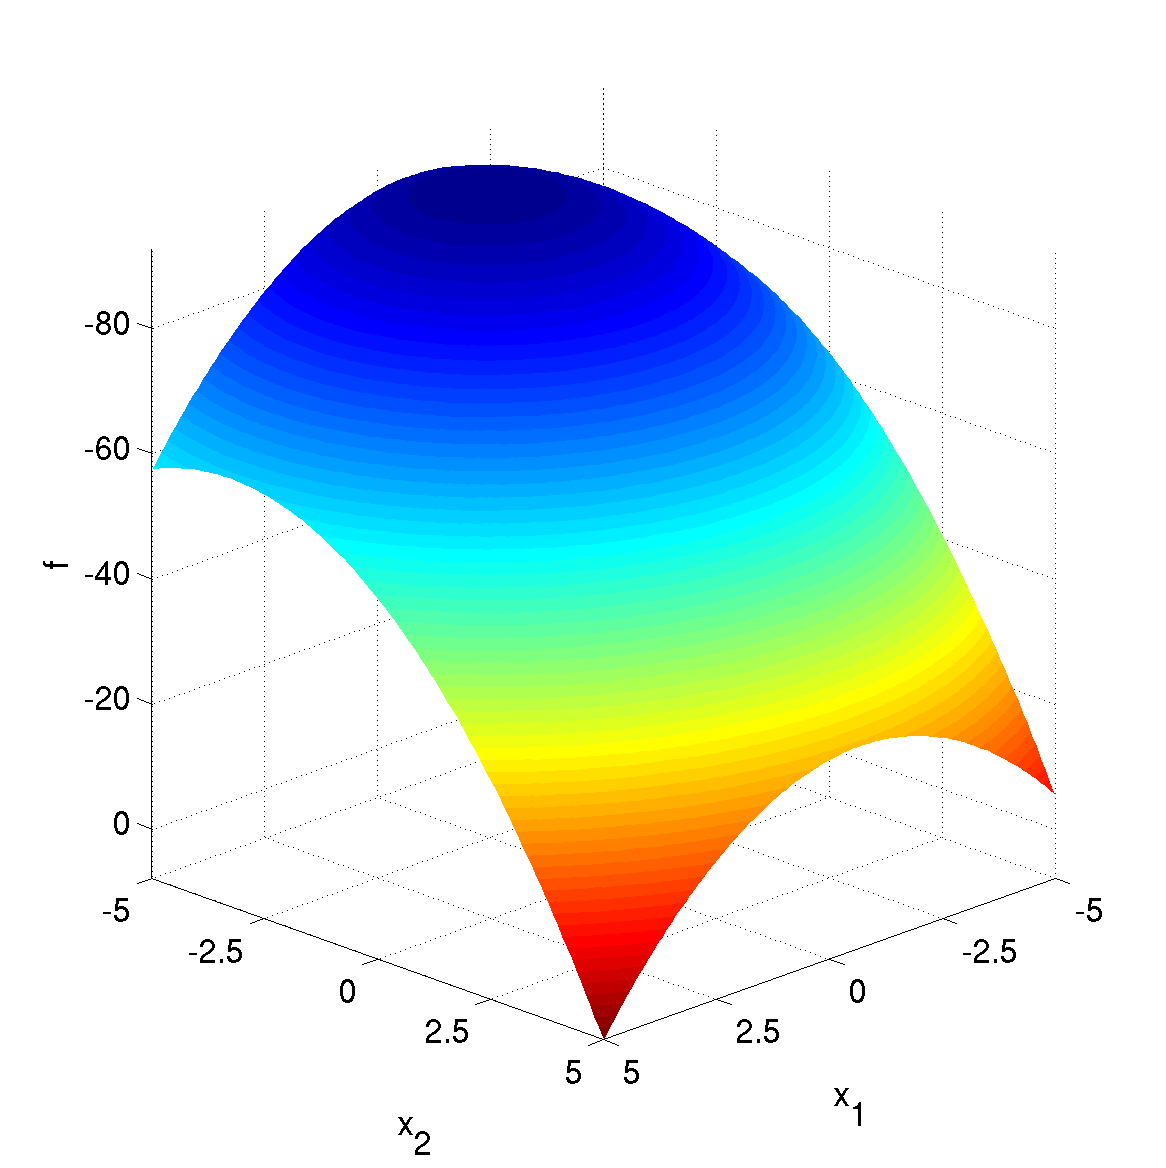
\includegraphics[page=1,width=0.108125\paperwidth]{graphics/problem_examples/bbob_functions/bbob_functions-00}%%
}{0.015}{0.49125}%
\locate{8}{%
\includegraphics[page=2,width=0.108125\paperwidth]{graphics/problem_examples/bbob_functions/bbob_functions-01}%%
}{0.138125}{0.49125}%
\locate{8}{%
\includegraphics[page=3,width=0.108125\paperwidth]{graphics/problem_examples/bbob_functions/bbob_functions-02}%%
}{0.26125}{0.49125}%
\locate{8}{%
\includegraphics[page=4,width=0.108125\paperwidth]{graphics/problem_examples/bbob_functions/bbob_functions-03}%%
}{0.384375}{0.49125}%
\locate{8}{%
\includegraphics[page=5,width=0.108125\paperwidth]{graphics/problem_examples/bbob_functions/bbob_functions-04}%%
}{0.5075}{0.49125}%
\locate{8}{%
\includegraphics[page=6,width=0.108125\paperwidth]{graphics/problem_examples/bbob_functions/bbob_functions-05}%%
}{0.630625}{0.49125}%
\locate{8}{%
\includegraphics[page=7,width=0.108125\paperwidth]{graphics/problem_examples/bbob_functions/bbob_functions-06}%%
}{0.75375}{0.49125}%
\locate{8}{%
\includegraphics[page=8,width=0.108125\paperwidth]{graphics/problem_examples/bbob_functions/bbob_functions-07}%%
}{0.876875}{0.49125}%
\locate{8}{%
\includegraphics[page=9,width=0.108125\paperwidth]{graphics/problem_examples/bbob_functions/bbob_functions-08}%%
}{0.015}{0.639166666666667}%
\locate{8}{%
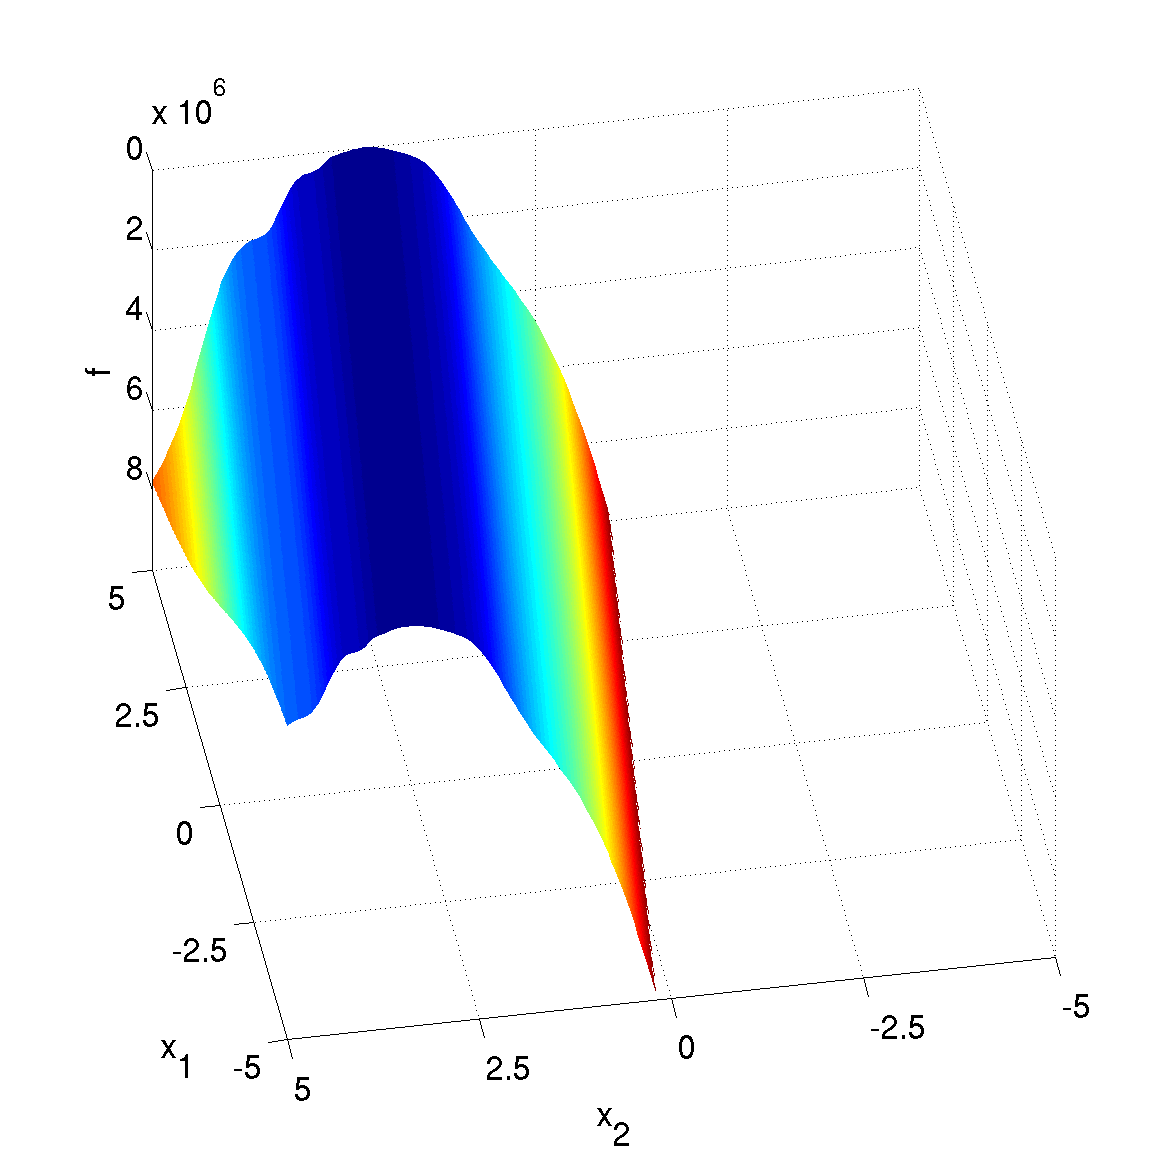
\includegraphics[width=0.108125\paperwidth]{graphics/problem_examples/bbob_functions/bbob_functions-09}%%
}{0.138125}{0.639166666666667}%
\locate{8}{%
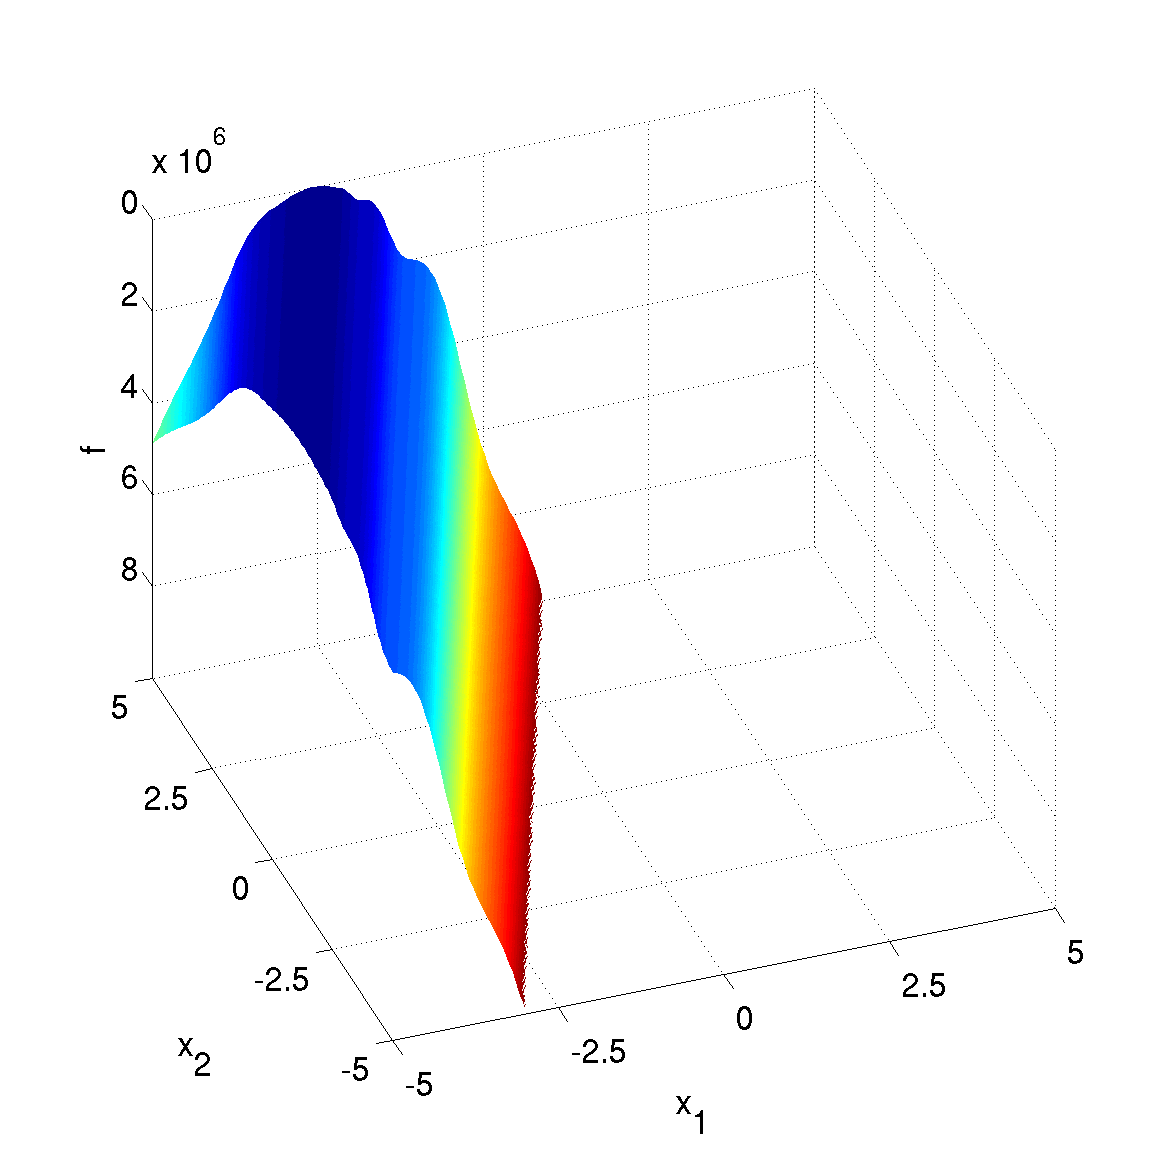
\includegraphics[width=0.108125\paperwidth]{graphics/problem_examples/bbob_functions/bbob_functions-10}%%
}{0.26125}{0.639166666666667}%
\locate{8}{%
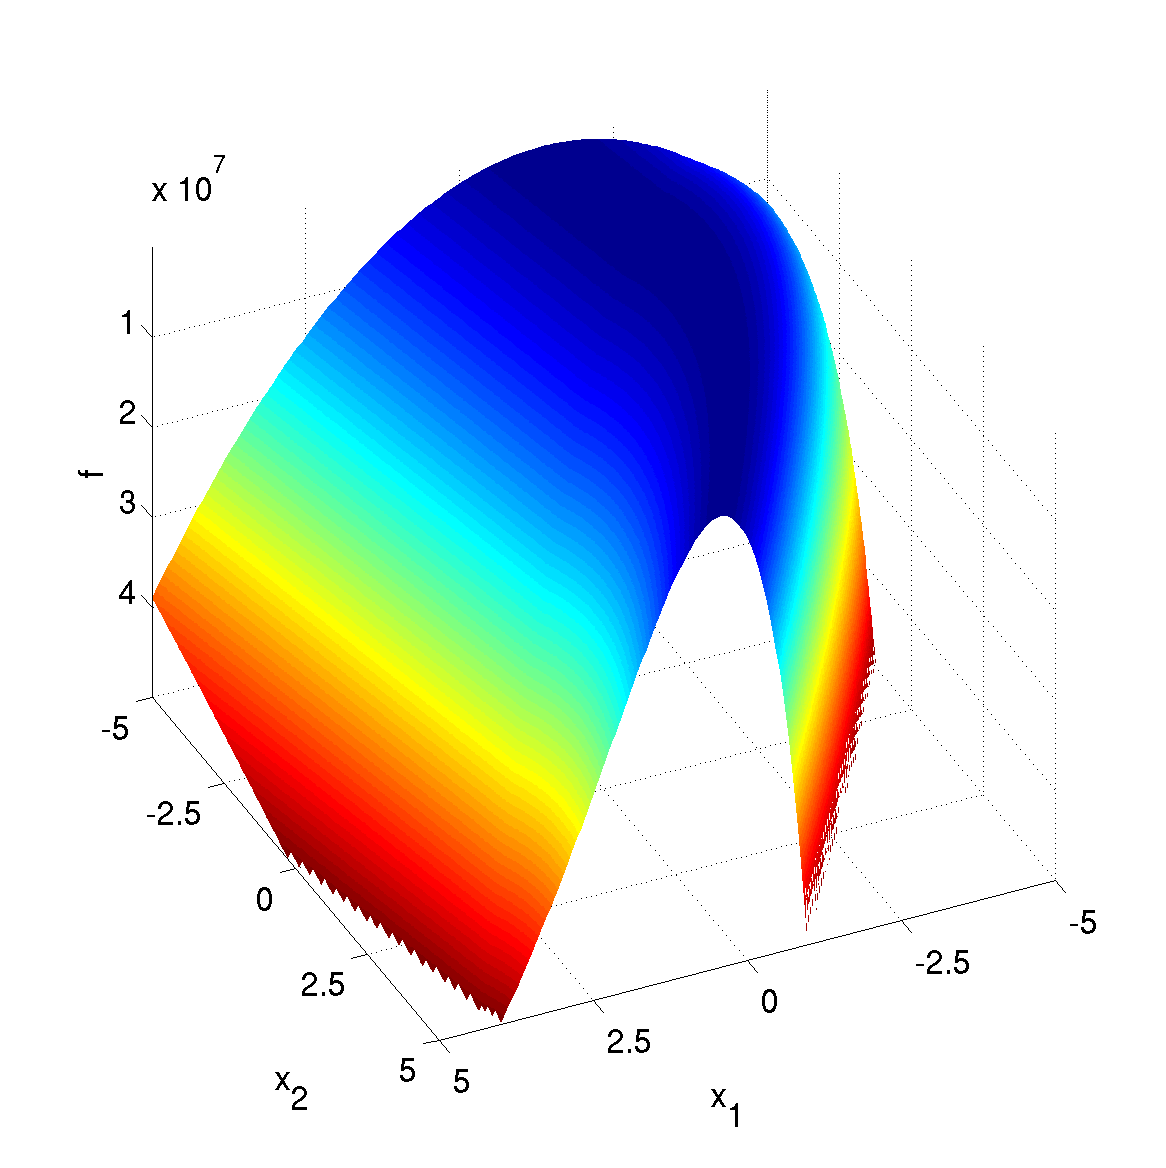
\includegraphics[width=0.108125\paperwidth]{graphics/problem_examples/bbob_functions/bbob_functions-11}%%
}{0.384375}{0.639166666666667}%
\locate{8}{%
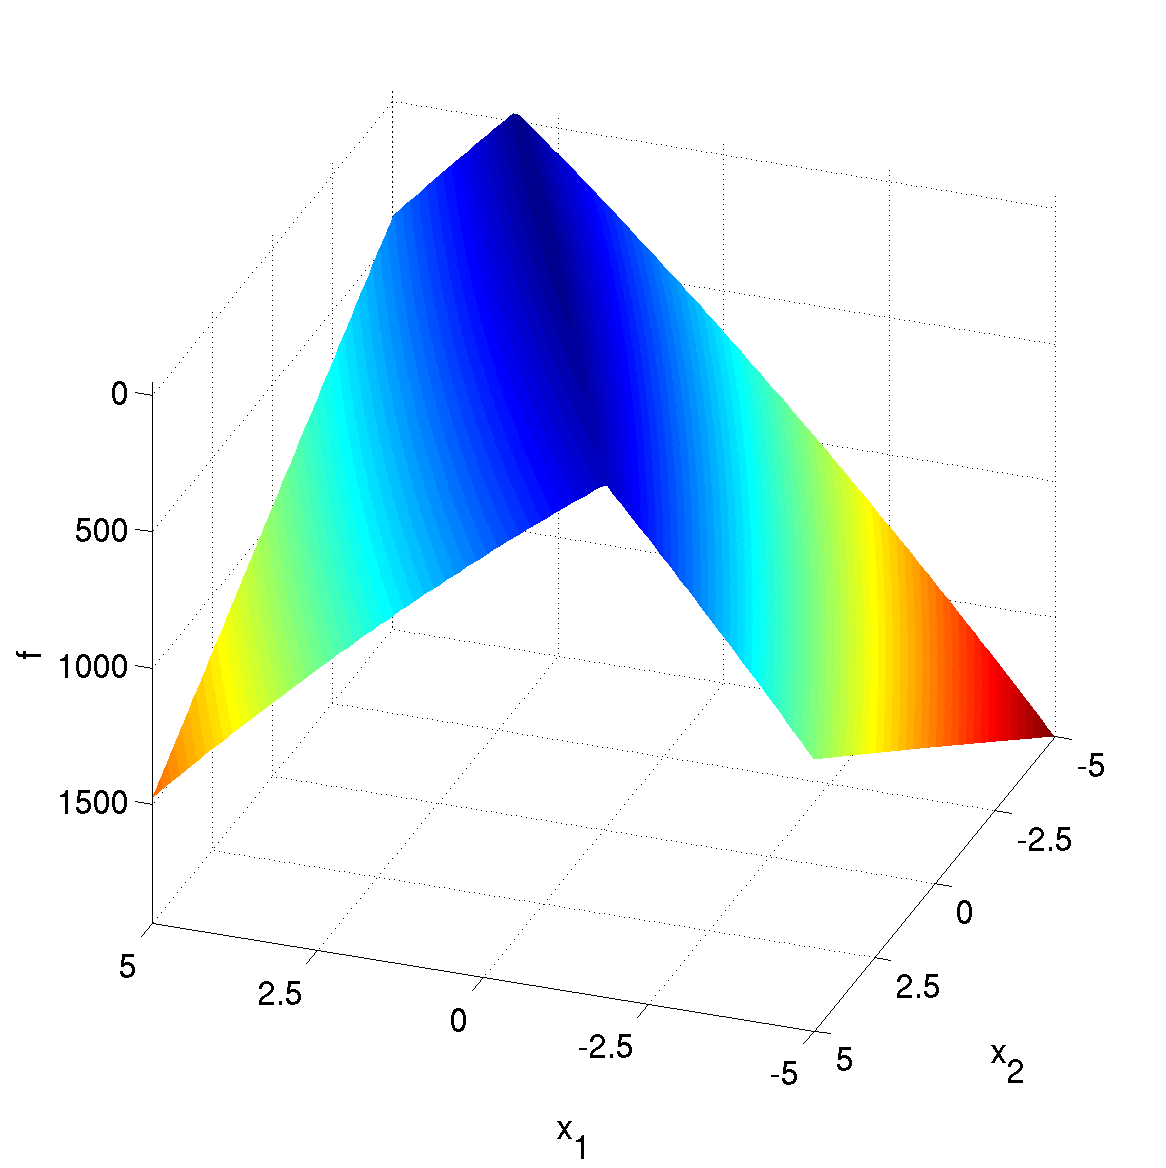
\includegraphics[width=0.108125\paperwidth]{graphics/problem_examples/bbob_functions/bbob_functions-12}%%
}{0.5075}{0.639166666666667}%
\locate{8}{%
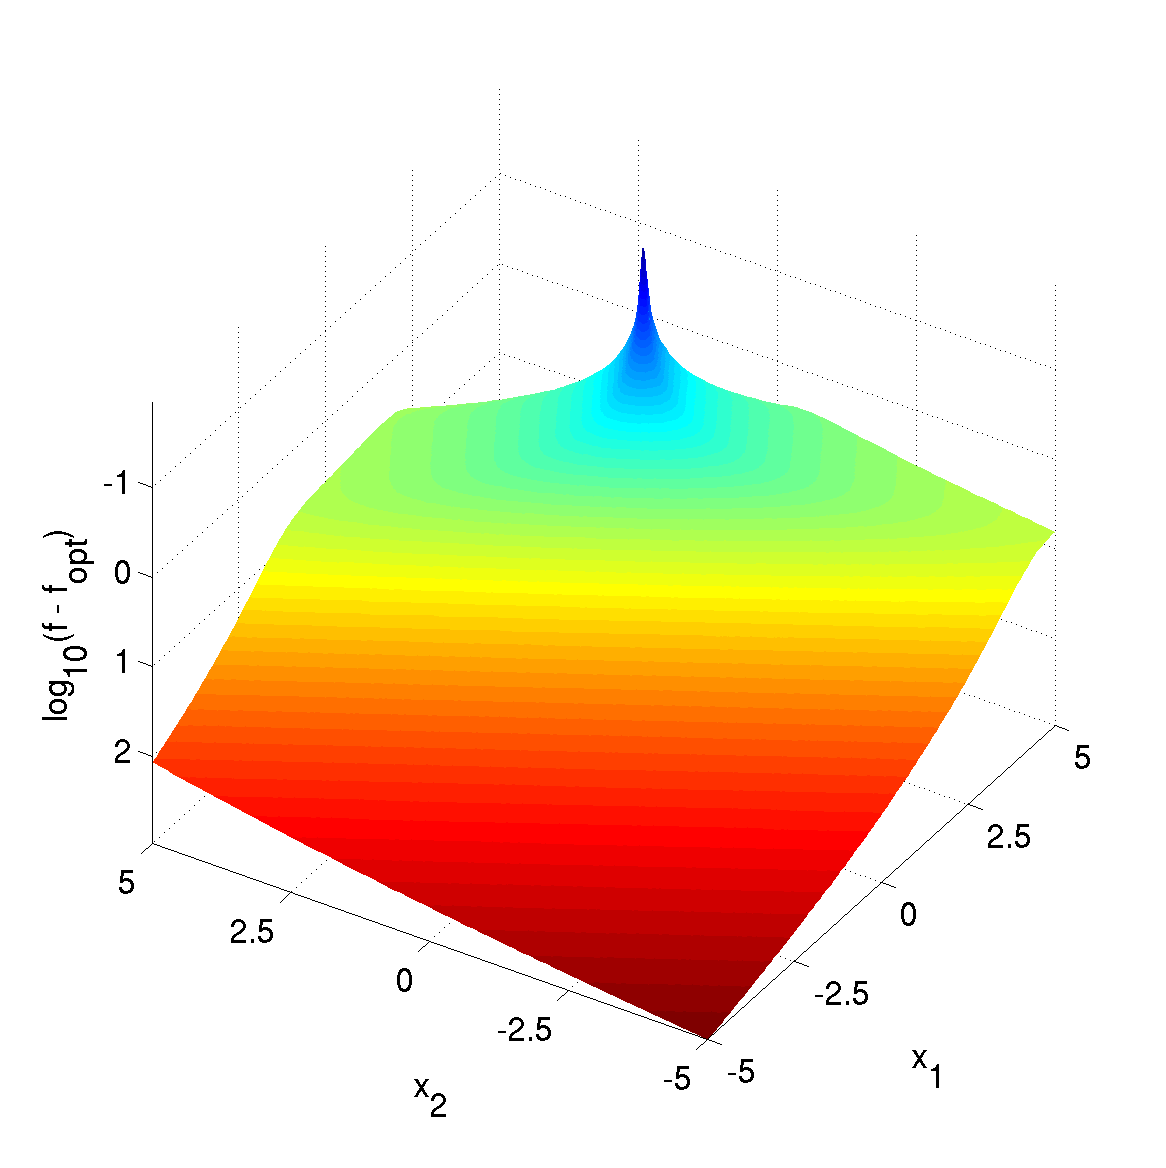
\includegraphics[width=0.108125\paperwidth]{graphics/problem_examples/bbob_functions/bbob_functions-13}%%
}{0.630625}{0.639166666666667}%
\locate{8}{%
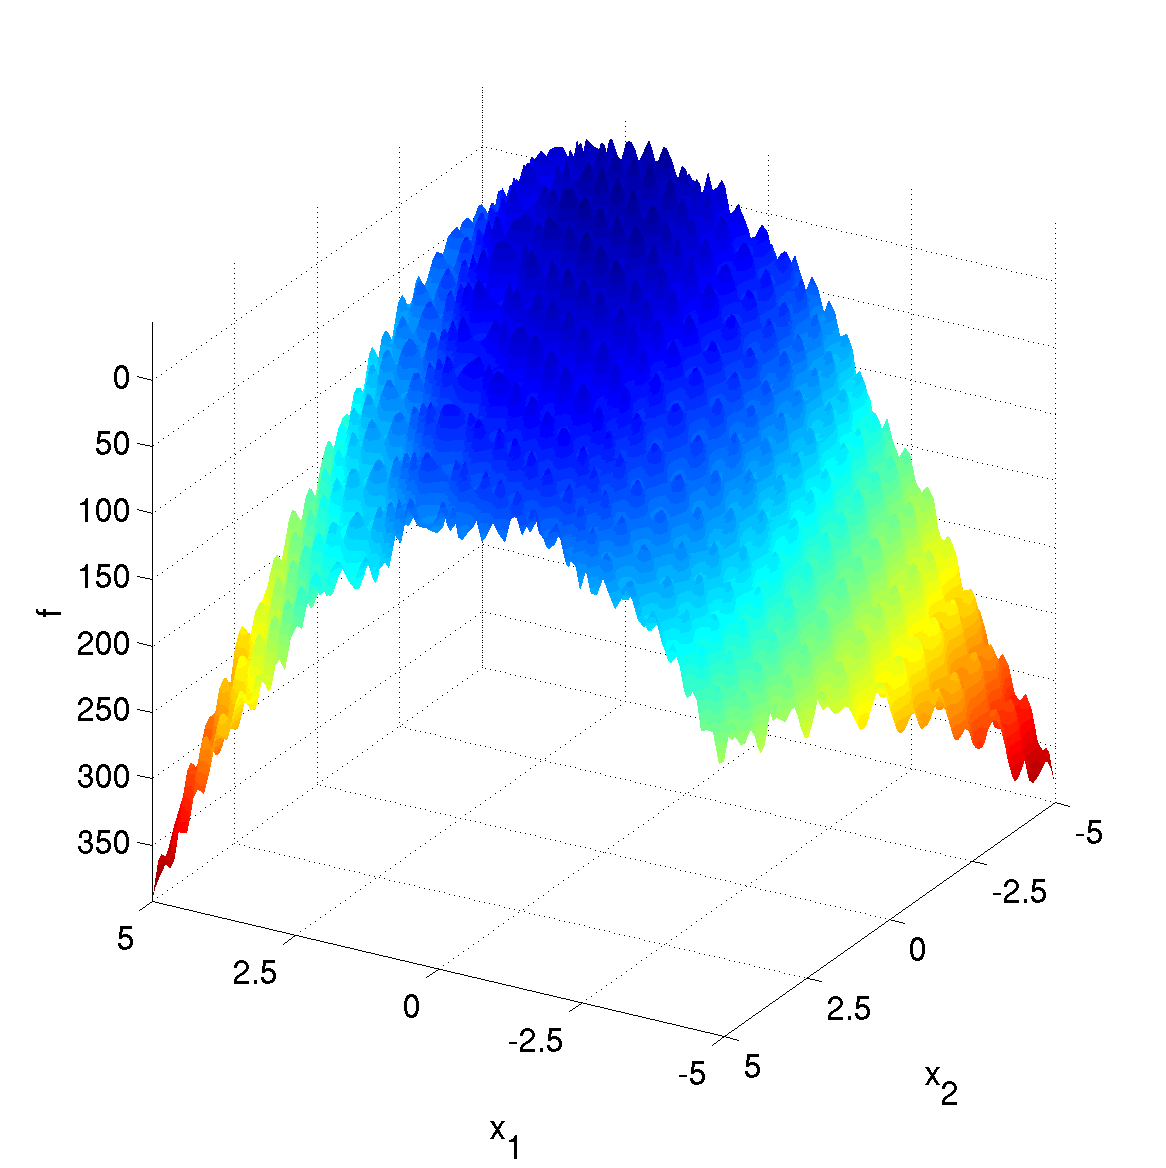
\includegraphics[width=0.108125\paperwidth]{graphics/problem_examples/bbob_functions/bbob_functions-14}%%
}{0.75375}{0.639166666666667}%
\locate{8}{%
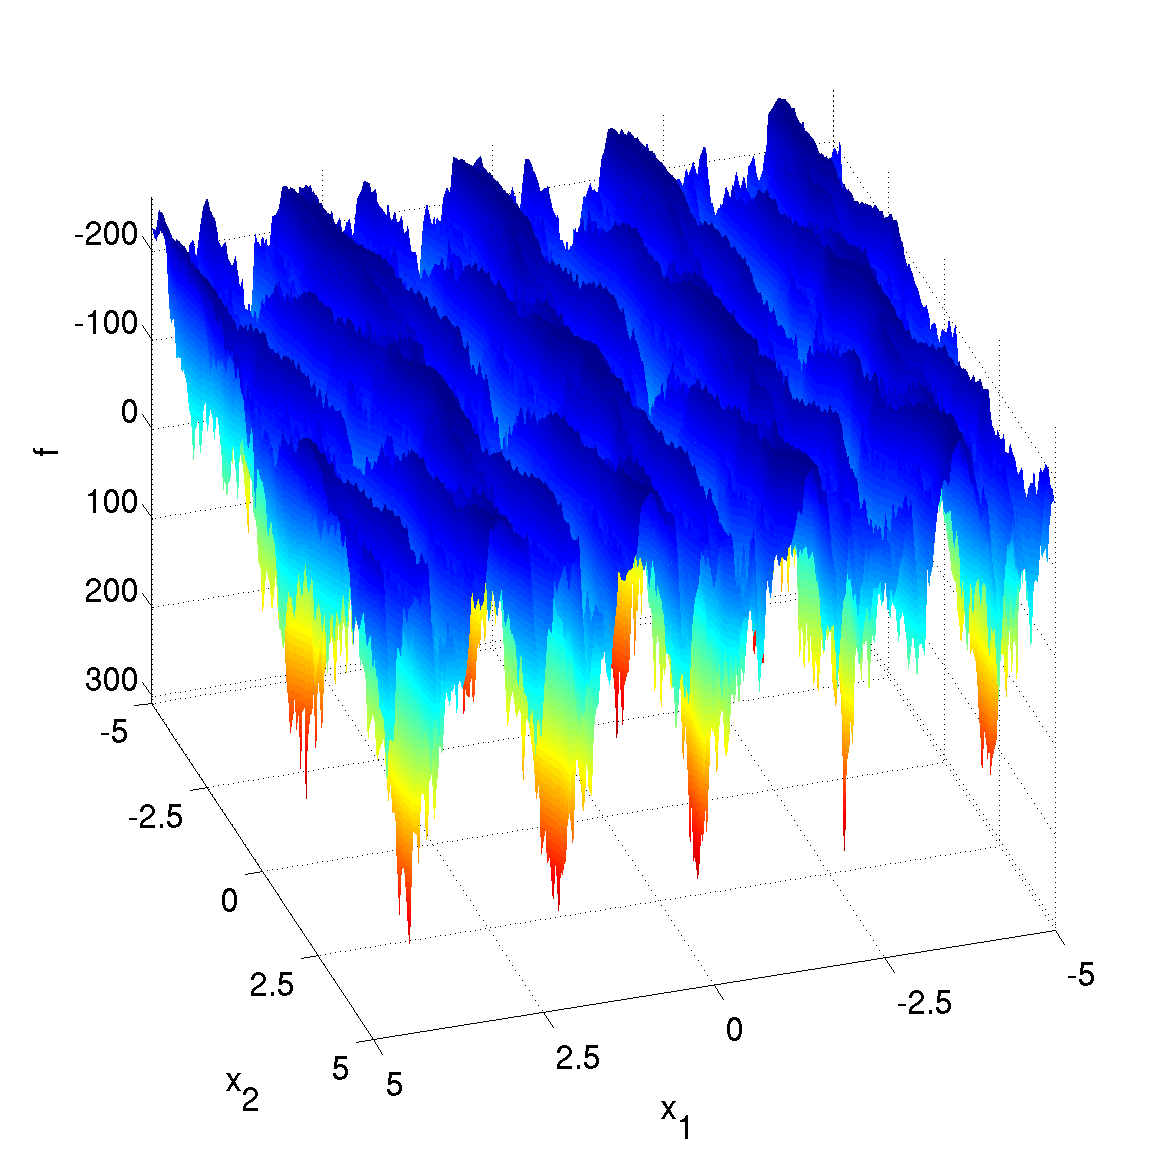
\includegraphics[width=0.108125\paperwidth]{graphics/problem_examples/bbob_functions/bbob_functions-15}%%
}{0.876875}{0.639166666666667}%
\locate{8}{%
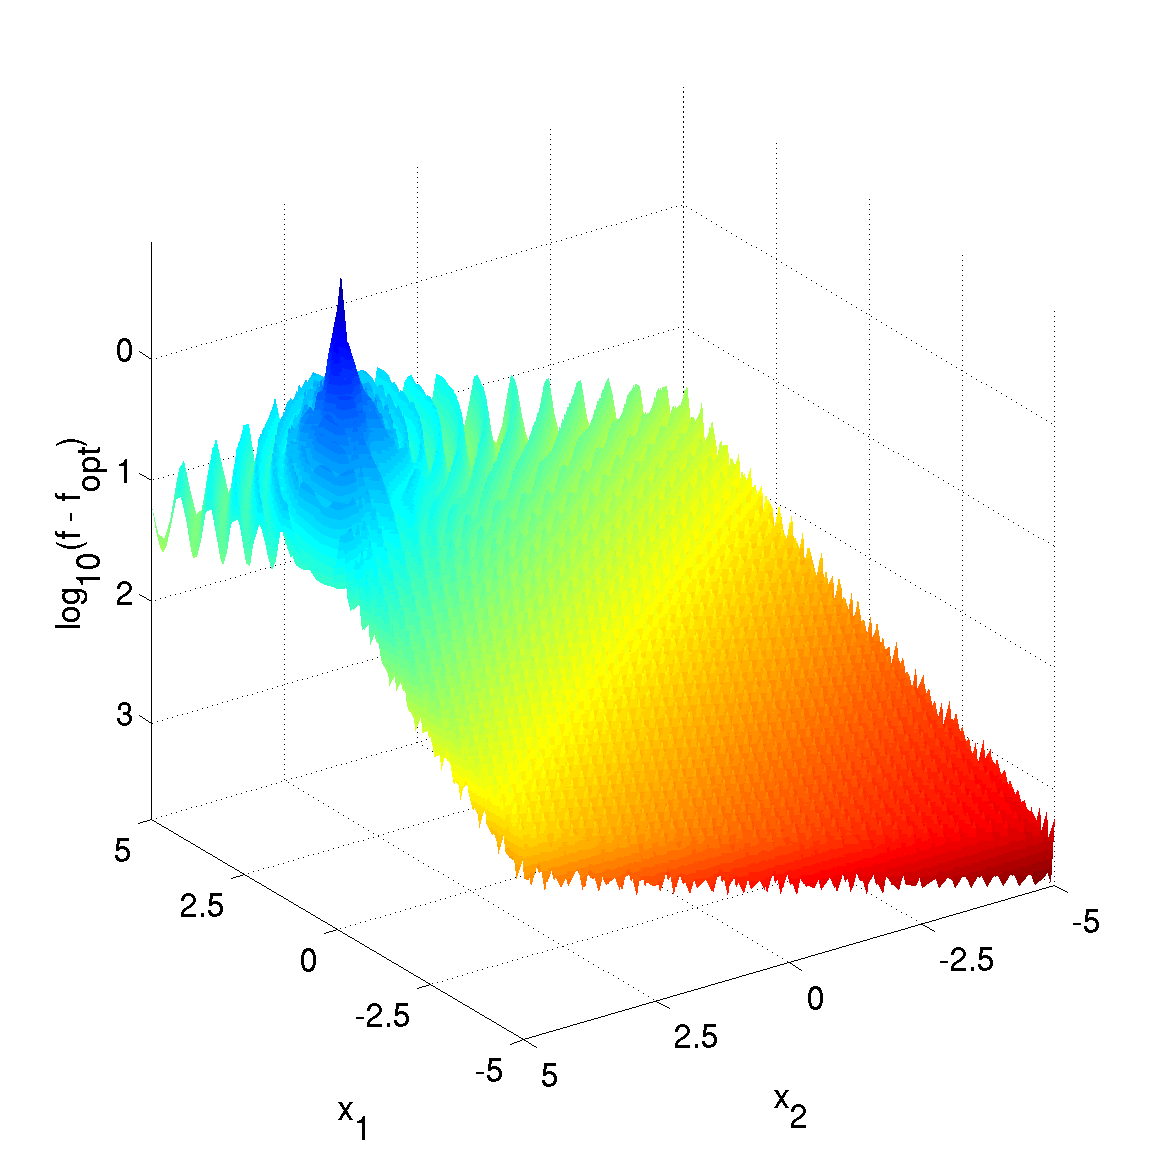
\includegraphics[width=0.108125\paperwidth]{graphics/problem_examples/bbob_functions/bbob_functions-16}%%
}{0.015}{0.787083333333333}%
\locate{8}{%
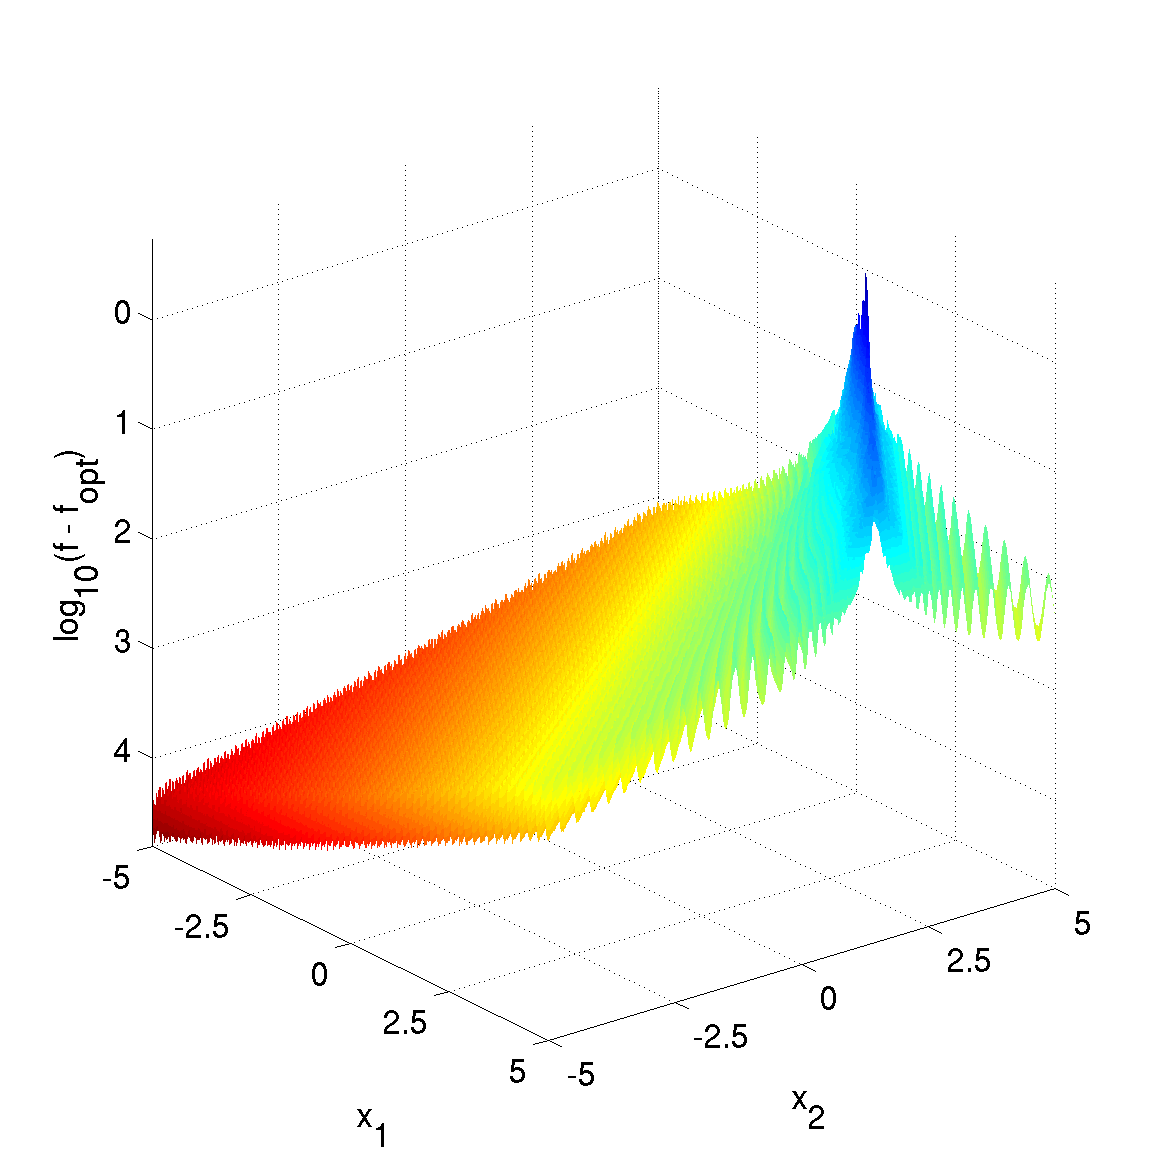
\includegraphics[width=0.108125\paperwidth]{graphics/problem_examples/bbob_functions/bbob_functions-17}%%
}{0.138125}{0.787083333333333}%
\locate{8}{%
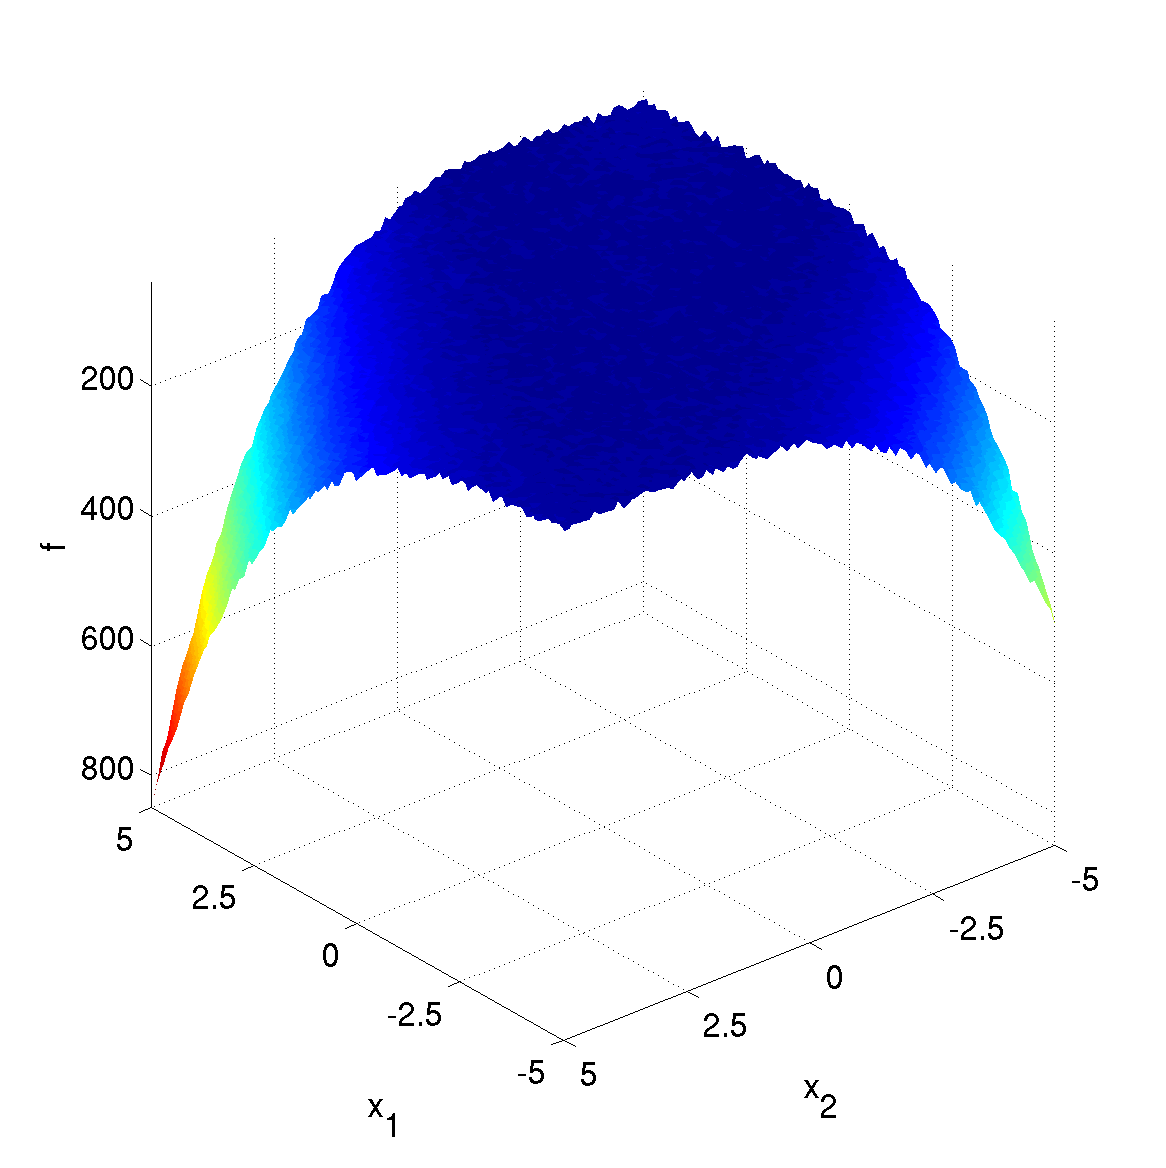
\includegraphics[width=0.108125\paperwidth]{graphics/problem_examples/bbob_functions/bbob_functions-18}%%
}{0.26125}{0.787083333333333}%
\locate{8}{%
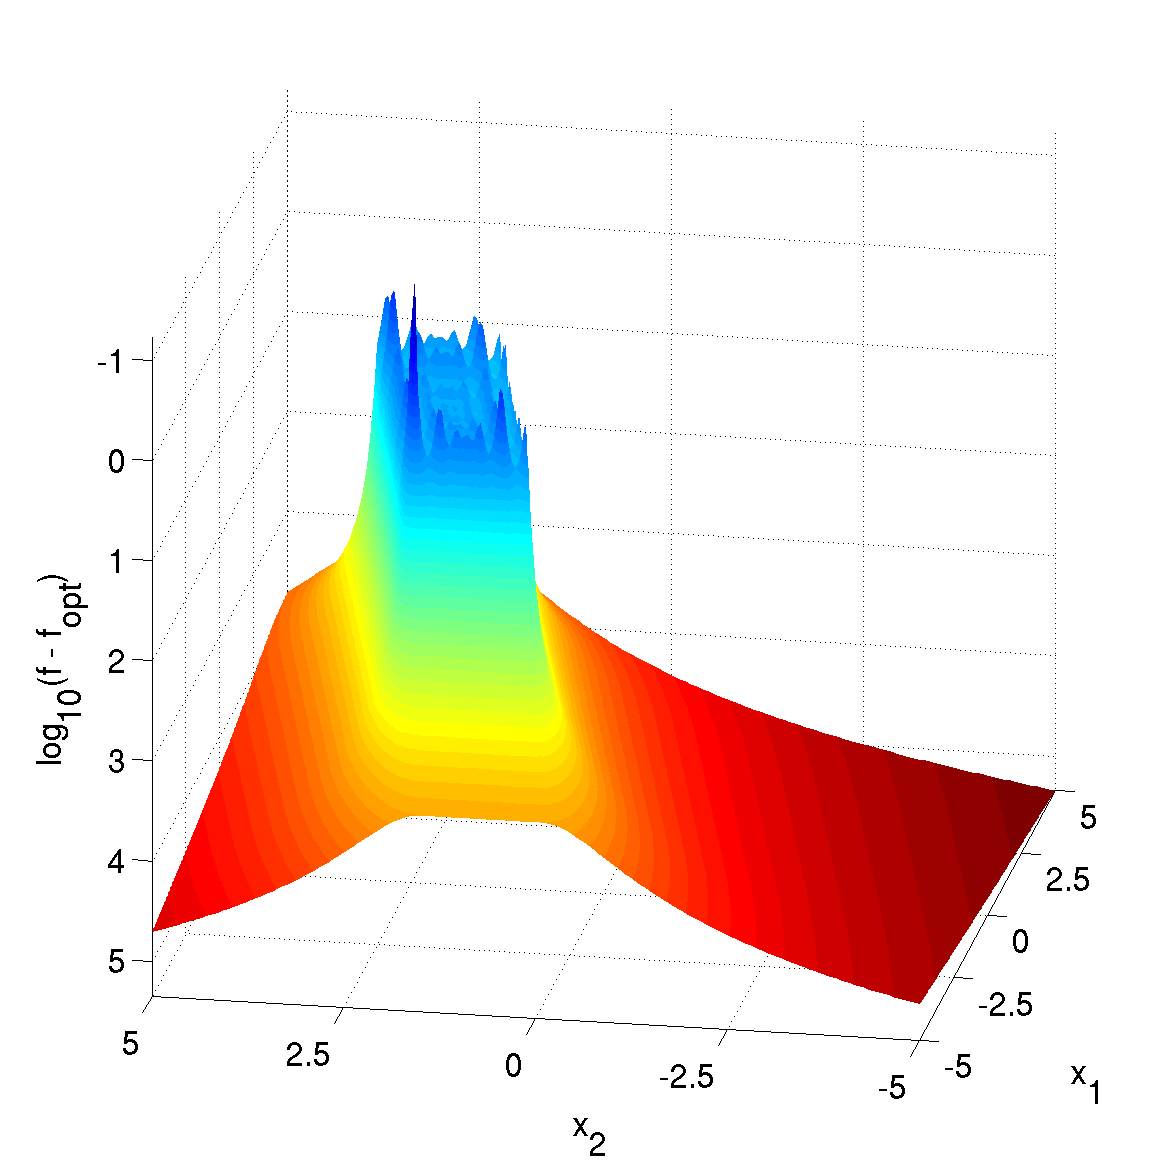
\includegraphics[width=0.108125\paperwidth]{graphics/problem_examples/bbob_functions/bbob_functions-19}%%
}{0.384375}{0.787083333333333}%
\locate{8}{%
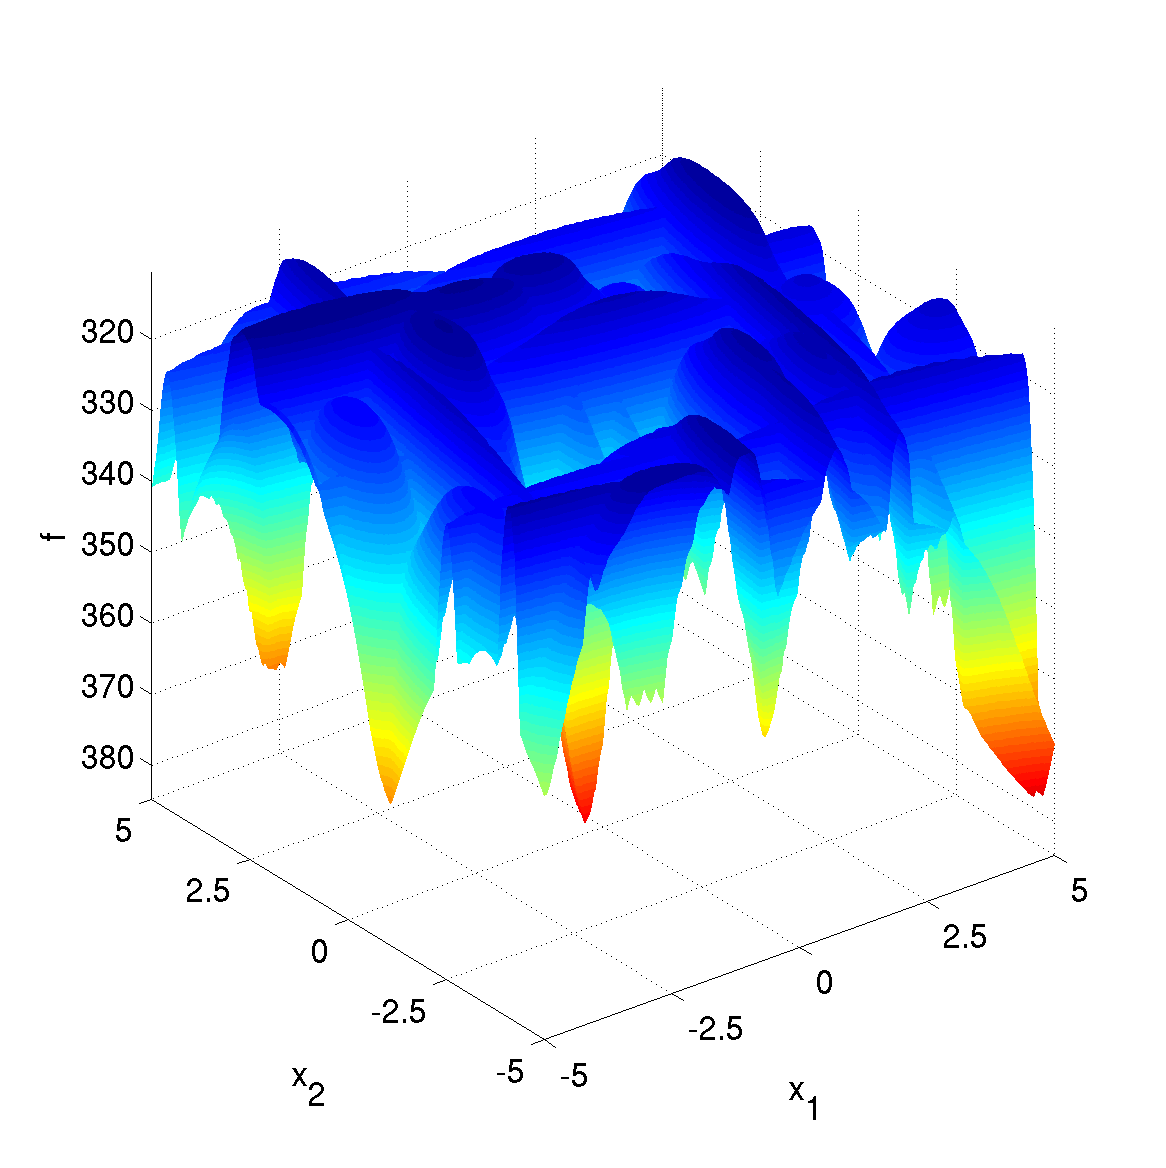
\includegraphics[width=0.108125\paperwidth]{graphics/problem_examples/bbob_functions/bbob_functions-20}%%
}{0.5075}{0.787083333333333}%
\locate{8}{%
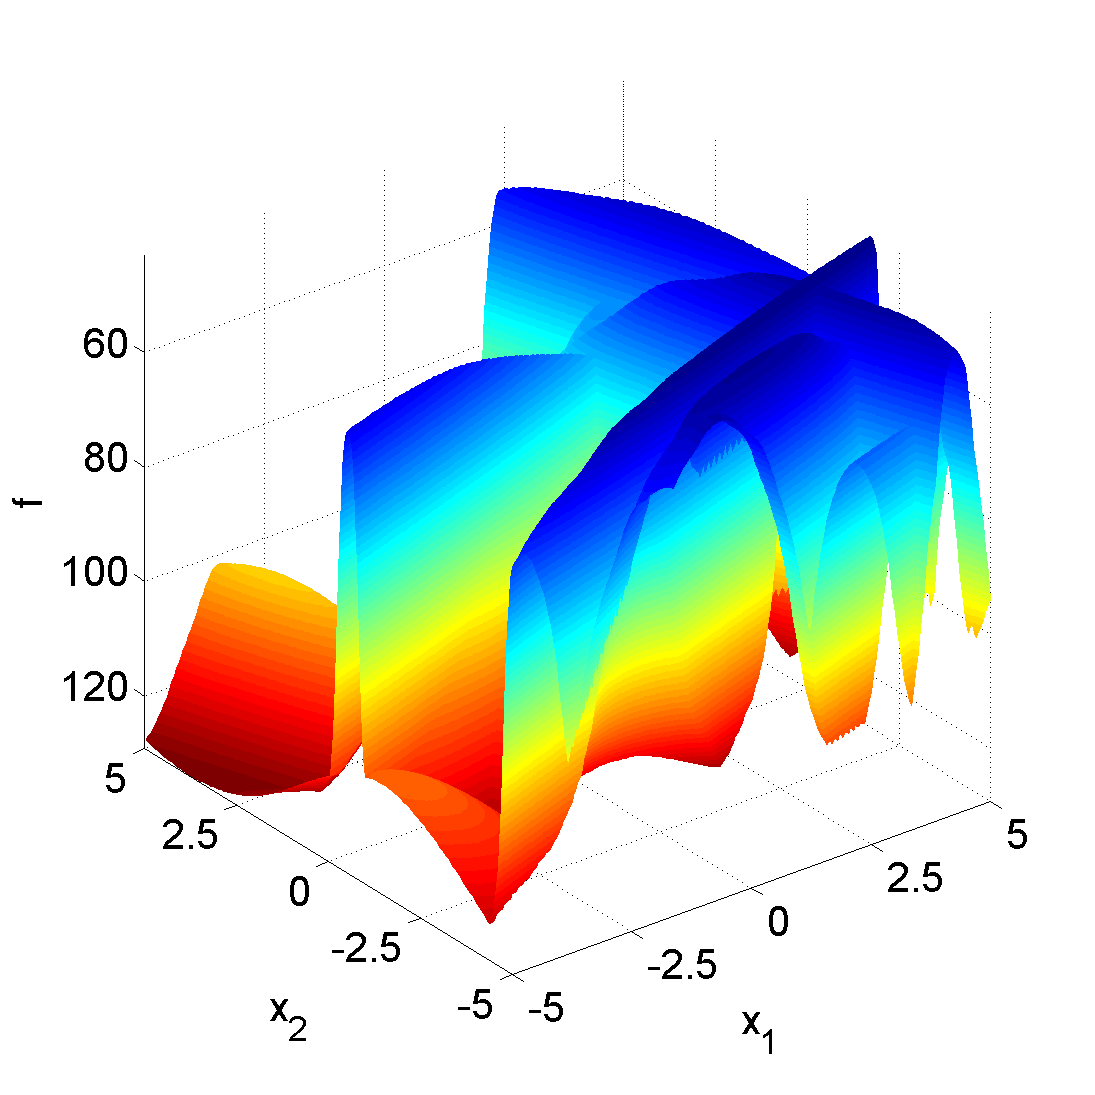
\includegraphics[width=0.108125\paperwidth]{graphics/problem_examples/bbob_functions/bbob_functions-21}%%
}{0.630625}{0.787083333333333}%
\locate{8}{%
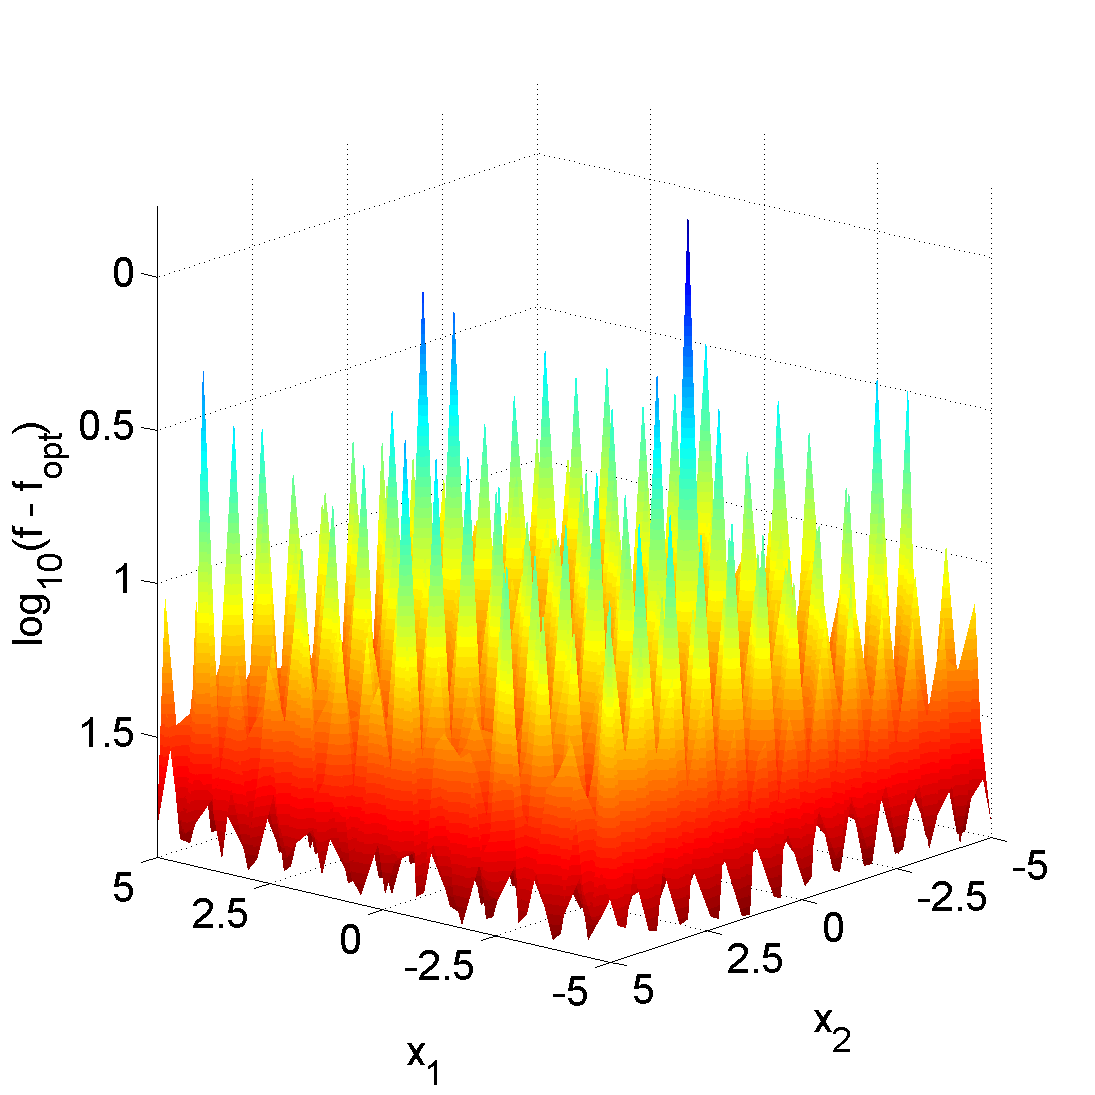
\includegraphics[width=0.108125\paperwidth]{graphics/problem_examples/bbob_functions/bbob_functions-22}%%
}{0.75375}{0.787083333333333}%
\locate{8}{%
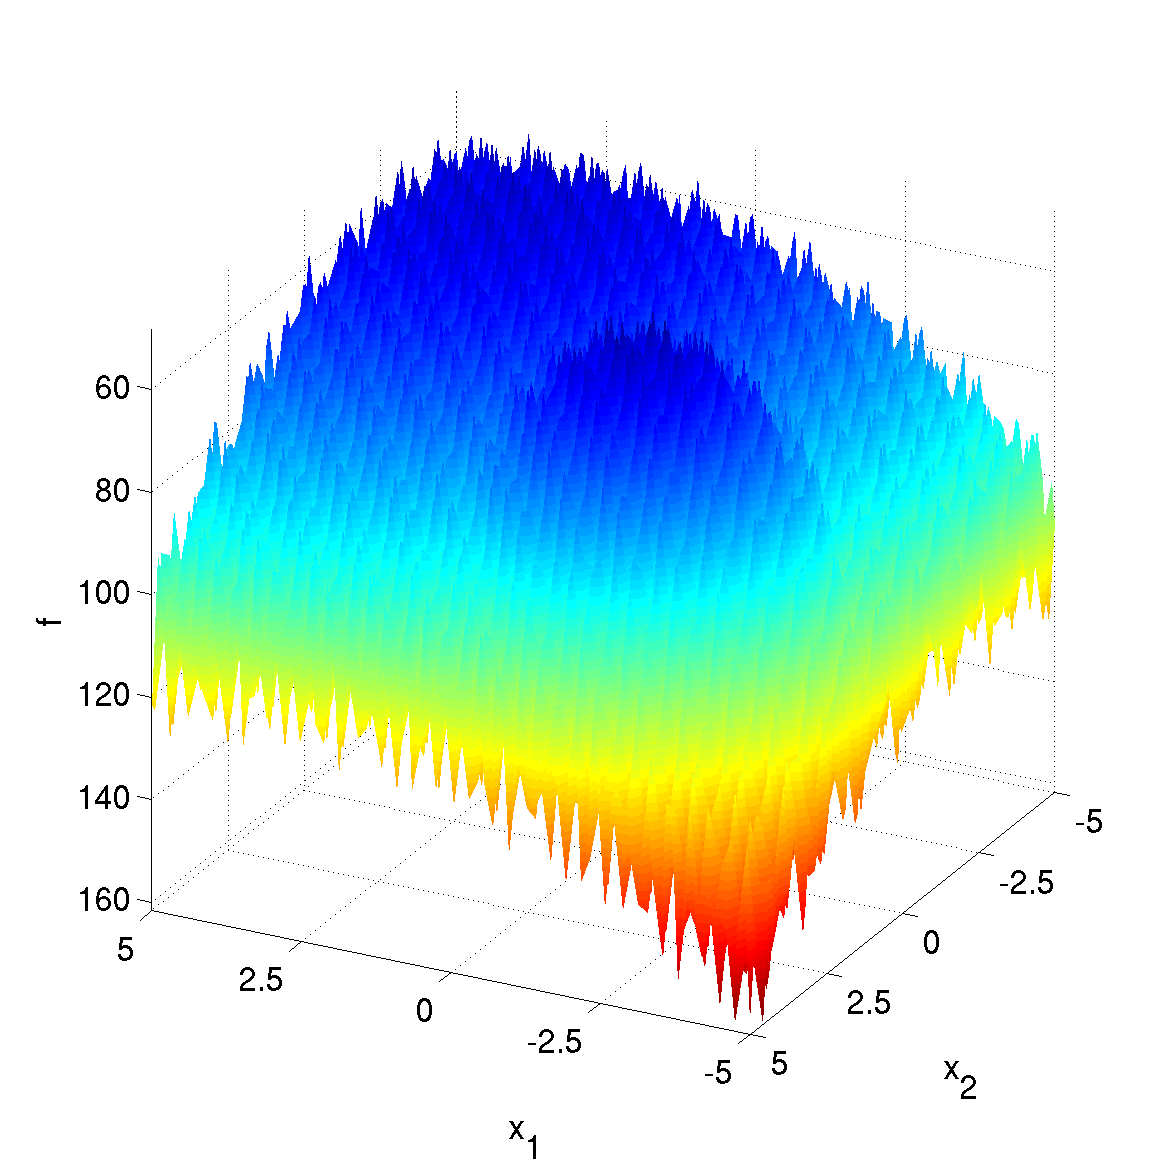
\includegraphics[width=0.108125\paperwidth]{graphics/problem_examples/bbob_functions/bbob_functions-23}%%
}{0.876875}{0.787083333333333}%
%
\end{frame}%
%
\section{Example Framework Scenario: Smart Manufacturing}%
%
\begin{frame}[t]%
\frametitle{What is Smart Manufacturing?}%
\textbf{\large{Smart Manufacturing}}\cite{DEPBS2012SMMIADDP}\dots%
\uncover<2->{%
\begin{itemize}%
\item has the goal of optimizing development, production, and logistics.%
\item<3-> employs computer control and high levels of adaptability in the multi-phase process of creating a product from raw material.
\item<4-> utilizes advanced information and manufacturing technologies to enable flexibility in production processes to address a dynamic market.%
\item<5-> requires increased workforce training for flexibility and use of the technology instead of simple repetitive tasks as in traditional manufacturing.%
\end{itemize}%
}%
%
\locateGraphic{}{width=0.8\paperwidth}{graphics/smart_manufacturing/smart_manufacturing}{0.1}{0.66}%
%
\end{frame}%
%
\begin{frame}[t]%
\frametitle{Industry~4.0\cite{HPO2016DPFI4S}}%
\locateGraphic{}{width=0.9\paperwidth}{graphics/industry_4_0/industry_4_0}{0.05}{0.22}%
\end{frame}%
%
\begin{frame}[t]%
\frametitle{Involved Technologies}%
\begin{itemize}%
\item Cyber-Physical Systems: deep connection between physical and software systems, often networks of interacting elements.\cite{KM2015DTAAOCSAS}%
\item<2-> Internet of Things: network enabling physical things to exchange data or being controlled, allowing a computer system to directly interact with the physical world.\cite{B2014IOTSFOBF}%
\item<3-> Cloud Computing: move data and computation into the cloud (not just storage, but also computational resources, applications).\cite{L2008CCL1WICCAAITPDP}%
\item<4-> Big Data: Collection, processing, and evaluation of huge amounts of data.\cite{M2014BDT5VEMK}%
\item<5-> These are some of the ingredients.\uncover<6->{ They do not make the production \alert{intelligent} yet.\uncover<7->{ They are technological enablers.}}%
\item<8-> \alert{Computational Intelligence and Optimization}\cite{aitoa,WGOEB,CWM2012VOEAFRWA}: automatic intelligent decisions, automated planning, scheduling, design, management, \dots%
\uncover<9->{~\dots\alert{can make systems \alert{intelligent}}}%
\end{itemize}%
\end{frame}%
%
%
\begin{frame}%
\frametitle{Relationship with Smart Manufacturing}%
\begin{itemize}%
\item So how is all of this related to smart manufacturing?%
\item<2-> No enterprise can waste money\uncover<3->{ or time\uncover<4->{ or material\uncover<5->{ or energy\uncover<6->{ or any other resource.}}}}%
\item<7-> An enterprise must try to make decisions which are optimial from the perspective of cost and resource consumption.%
\item<8-> An enterprise must strive to improve its processes and products.%
\item<9-> An enterprise should want to have \only<-12>{tools}\only<13->{\alert{software}} that can automatically make good suggestions\uncover<10->{, which can save costs and resources for the daily operations\uncover<11->{, the long term planning\uncover<12->{, and/or even its product/organizational development.}}}%
%
\item<14-> All kinds of the previously mentioned problems can occur in manufacturing.%
\item<15-> For example, logistics exist inside and outside a company, and even on the factory floor!%
\end{itemize}%
\end{frame}
%
%
\begin{frame}%
\frametitle{Examples from Smart Manufacturing}%
\begin{itemize}%
\item Our factory receives a set of customer orders and we need to assign them to workers/machines in order to complete them in time.%
\item<2-> We need to plan which worker works on which machine or task based on preferences, regulations, and efficiency.%
\item<3-> We need to plan the purchase of raw material based on expected production orders.%
\item<4-> We need to store items in the warehouse efficiently for fast access.%
\item<5-> We need to cut a large piece of cloth into smaller pieces for clothing production while minimizing waste.%
\item<6-> We need to route inter-workshop or inter-workstation material transportation.%
\item<7-> We need to plan maintenance of machinery.%
\item<8-> \dots%
\end{itemize}%
\end{frame}%
%
\begin{frame}%
\frametitle{Examples from Smart Manufacturing}%
\locateGraphic{1}{width=0.99\paperwidth}{graphics/five_aspects/five_aspects}{-0.0001}{0.17}%
\uncover<2->{%
\begin{itemize}%
\item When developing a real-world application of optimization, there are two issues\uncover<3->{:%
\begin{enumerate}%
\item Developing and implementing a good algorithm that can solve the problem at hand\uncover<4->{ and}%
\item<4-> integrating this implementation into the existing software ecosystem.
\end{enumerate}%
}%
\item<5-> We focus only on the first of the two issues: optimization algorithms and their implementation.%
\end{itemize}%
}%
\end{frame}%
%
%
\section{Exact vs.\ Heuristic Algorithms}%
%
%
\begin{frame}[t]%
\frametitle{Exact vs.\ Heuristic Algorithms}%
\begin{itemize}%
\item In optimization, there exist \alert{exact} and \alert{heuristic} algorithms.%
%
\item<2-> Let's again look at the classical Traveling Salesman Problem (TSP).%
\only<3-5,7->{%
\begin{itemize}%
\only<-5>{\item Clearly, there is (at least) one shortest tour.}%
\only<-8>{\item<5-> \only<-5>{Theory proofs that the time to find this tour may grow exponentially with the number of cities we want to visit in the worst case.\cite{LLRKS1993SASAAC,CPW1998AROMSCAAA,C1971TCOTPP,K1972RACP,A2008TLOQC}}%
\only<7->{Finding the best tour (what exact algorithms do) may take too long.}}%
\only<-9>{\item<8-> But we can find just \alert{some} tour very quickly.}%
\only<-11>{\item<9-> Of course the quality of that tour will be lower\only<10>{: the tour will be longer than the best one}.}%
\only<-12>{\item<11-> Is there something inbetween?}%
\only<-13>{\item<12-> (Meta-)Heuristic optimization algorithms try to find solutions which are as good as possible as fast as possible.}%
\item<13-> \alert{Optimization often means to make a trade-off between solution quality and runtime\only<14->{ and \alert{development time (the time from the definition of the problem until we have a software for producing solutions)}}.}%
\end{itemize}%
}%
\end{itemize}%
%
\strut\\\strut\\\strut\\\strut\\\strut\\\strut\\\strut\\\strut\\\strut\\\strut\\\strut\\\strut\\\strut\\\strut\\\strut\\\strut\\\strut\\\strut\\\strut%
%
%
\locateGraphic{2-3}{width=0.6\paperwidth}{graphics/problem_examples/tsp/tsp_china}{0.2}{0.29}%
\locateGraphic{4-5}{width=0.74\paperwidth}{graphics/runtime_quality_tradeoff/runtime_quality_tradeoff_1}{0.13}{0.42}%
\locateGraphic{6}{width=0.98\paperwidth}{graphics/function_growth/function_growth}{0.01}{0.27}%
\locateGraphic{7}{width=0.74\paperwidth}{graphics/runtime_quality_tradeoff/runtime_quality_tradeoff_2}{0.13}{0.42}%
\locateGraphic{8}{width=0.74\paperwidth}{graphics/runtime_quality_tradeoff/runtime_quality_tradeoff_3}{0.13}{0.42}%
\locateGraphic{9-10}{width=0.74\paperwidth}{graphics/runtime_quality_tradeoff/runtime_quality_tradeoff_4}{0.13}{0.42}%
\locateGraphic{11}{width=0.74\paperwidth}{graphics/runtime_quality_tradeoff/runtime_quality_tradeoff_5}{0.13}{0.42}%
\locateGraphic{12}{width=0.74\paperwidth}{graphics/runtime_quality_tradeoff/runtime_quality_tradeoff_6}{0.13}{0.42}%
\locateGraphic{13-14}{width=0.74\paperwidth}{graphics/runtime_quality_tradeoff/runtime_quality_tradeoff_7}{0.13}{0.42}%
\locateGraphic{15}{width=0.74\paperwidth}{graphics/runtime_quality_tradeoff/runtime_quality_tradeoff_8}{0.13}{0.42}%
\end{frame}%
%
\begin{frame}[t]%
\frametitle{Metaheuristics}%
%
\begin{itemize}%
\item Heuristics are often simple, specialized algorithms that create an approximate solution for a very specific, narrow class of problems, say a TSP with cities in the Euclidean plane.%
\item<2-> However, there are many different optimization problems\only<3-4>{ and often we won't see a ``pure'' TSP in practice\only<4>{, there usually will be additional constraints and restrictions or multiple cars etc}}.%
\item<5-> Should we develop a completely new method for each problem?%
\item<6-> No. We want general algorithms that can be adapted to different problems.%
\uncover<8->{ (also to reduce the development time\only<-8>{)}\uncover<9->{ {\dots} we often want a prototype quickly and can add more complex logic later)}}%
\end{itemize}%
%
\uncover<7->{%
%
\begin{definition}[Metaheuristic]%
A metaheuristic is a method for solving a general class of problems. %
It combines objective functions or heuristics in an abstract and hopefully efficient way, usually by treating them as black box-procedures.\cite{aitoa,WGOEB,GK2003HOM,MF2004HTSIMH}%
\end{definition}%
}%
\end{frame}%
%
%
\section{Summary and Outlook}%
%
\begin{frame}%
\frametitle{Summary and Outlook}%
%
\begin{itemize}%
\item There is a wide variety of optimization problems in Smart Manufacturing.%
\item<2-> There also exists a wide variety of optimization algorithms.%
\item<3-> There are many different applications and almost all have specific requirements.%
\item<4-> There is no (and can never be a) single, perfect algorithm to solve all of them.\cite{WM1995NFLTFS,WM1997NFLTFO,AT2009CLAFPTDOOOA,AT2010CLAFPTDOOOA}%
\item<5-> Experience is needed: How do I recognize an optimization problem? How can I quickly make a software that can solve it?%
\item<6-> We will try to get a good perspective and understanding of the very basics needed to navigate in the domain of optimization.%
\item<7-> The goal is to be able to recognize and identify optimization problems as they occur in many fields, especially in Intelligent Manufacturing scenarios, and to develop basic algorithms to solve them.%
\end{itemize}%
%
\end{frame}%
%
\endPresentation%
\end{document}%%
\endinput%
%
